\problemname{Chalmers mörka källare}
Du är på väg till finalen i Programmeringsolympiaden. 
Dessvärre har du gått vilse i Chalmers mörka källare. 
Ditt lokalsinne är inte på topp, och det hjälper inte att källaren är utformad på ett mycket underligt sätt.

\begin{centering}
  \begin{figure}[h]
    \centering
    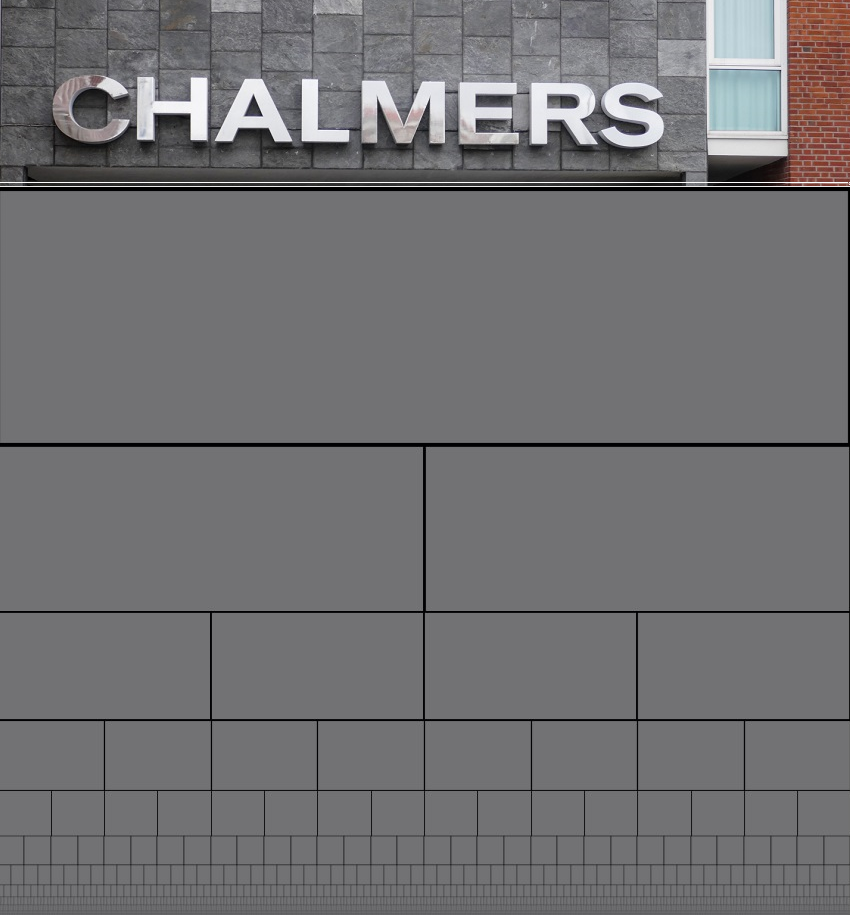
\includegraphics[scale=0.6]{chalmers_dark_chambers.png}
    \caption{Chalmers mörka källare...}
  \end{figure}
\end{centering}

Källaren består av $2 \leq N \leq 1000$ våningar. 
På bottenplan finns ett enda stort rum.
Alla andra rum har ett rum direkt ovanför sig.
När du går ner en våning blir rummen hälften så stora.
Under varje rum $i$ finns upp till två rum $l_i$ och $r_i$ som är precis hälften så stora.
Det är också möjligt att bara ett av $l_i$ och $r_i$ finns, eller att inget av dem finns. 
Du kan ta dig mellan två rum genom en dörr om de ligger precis bredvid varandra, 
eller via en trappa om det ena ligger direkt över det andra.
Du kan ta dig till alla rum från bottenplan utan att gå igenom dörrar.
Du befinner dig just nu i något rum i källaren, och du vet att rummet där finalen hålls också ligger i källaren.

En \emph{väg} är en sekvens av steg till närliggande rum.
För någon väg $v$ från rummet du befinner dig i till rummet finalen hålls i,
låt $A_v$ vara antalet gånger du går genom en dörr,
och $B_v$ antalet gånger du går upp eller ner för en trappa.
Vägens \emph{längd} definieras som summan $L_v = A_v + B_v$.
Du vill nu ta dig till finalen. Till din hjälp har du appen Campus Maps.
Campus Maps är programmerad för att hitta längden på den väg till din destination,
där antalet trappor du behöver gå upp eller ned för minimeras.
Av alla möjliga vägar $v$ till rummet där finalen hålls kommer appen att hitta de som minimerar värdet på $B_v$.
Av alla dessa vägar kommer appen sedan välja den som minimerar värdet på $L_v$.
Den kommer sedan ge dig värdet $L_v$, längden på denna vägen.

Eftersom appen tar väldigt lång tid att ladda så hinner du kolla i den som mest $500$ gånger. 
Du hinner inte heller passera fler än $5000$ rum.

\begin{centering}
  \begin{figure}[h]
      \centering
      \begin{subfigure}
        \centering
        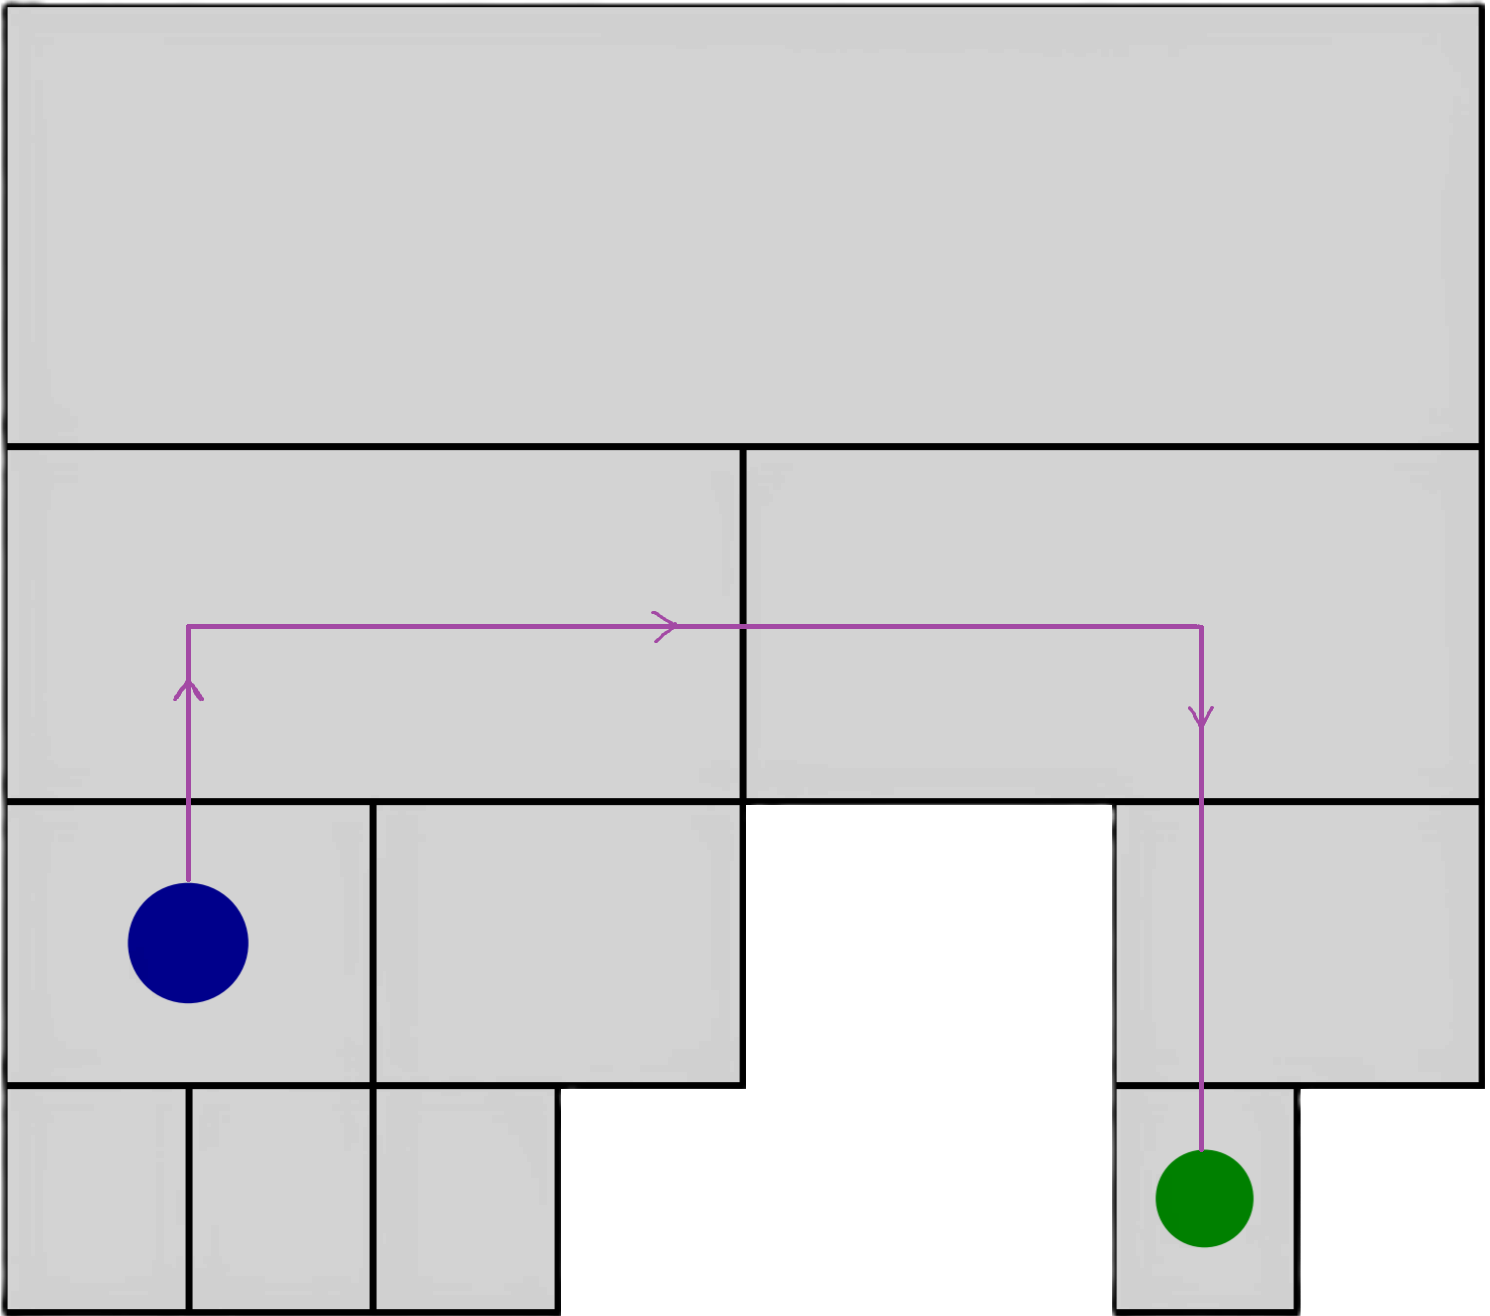
\includegraphics[scale=0.8]{sample1.png}
      \end{subfigure}
      \begin{subfigure}
        \centering
        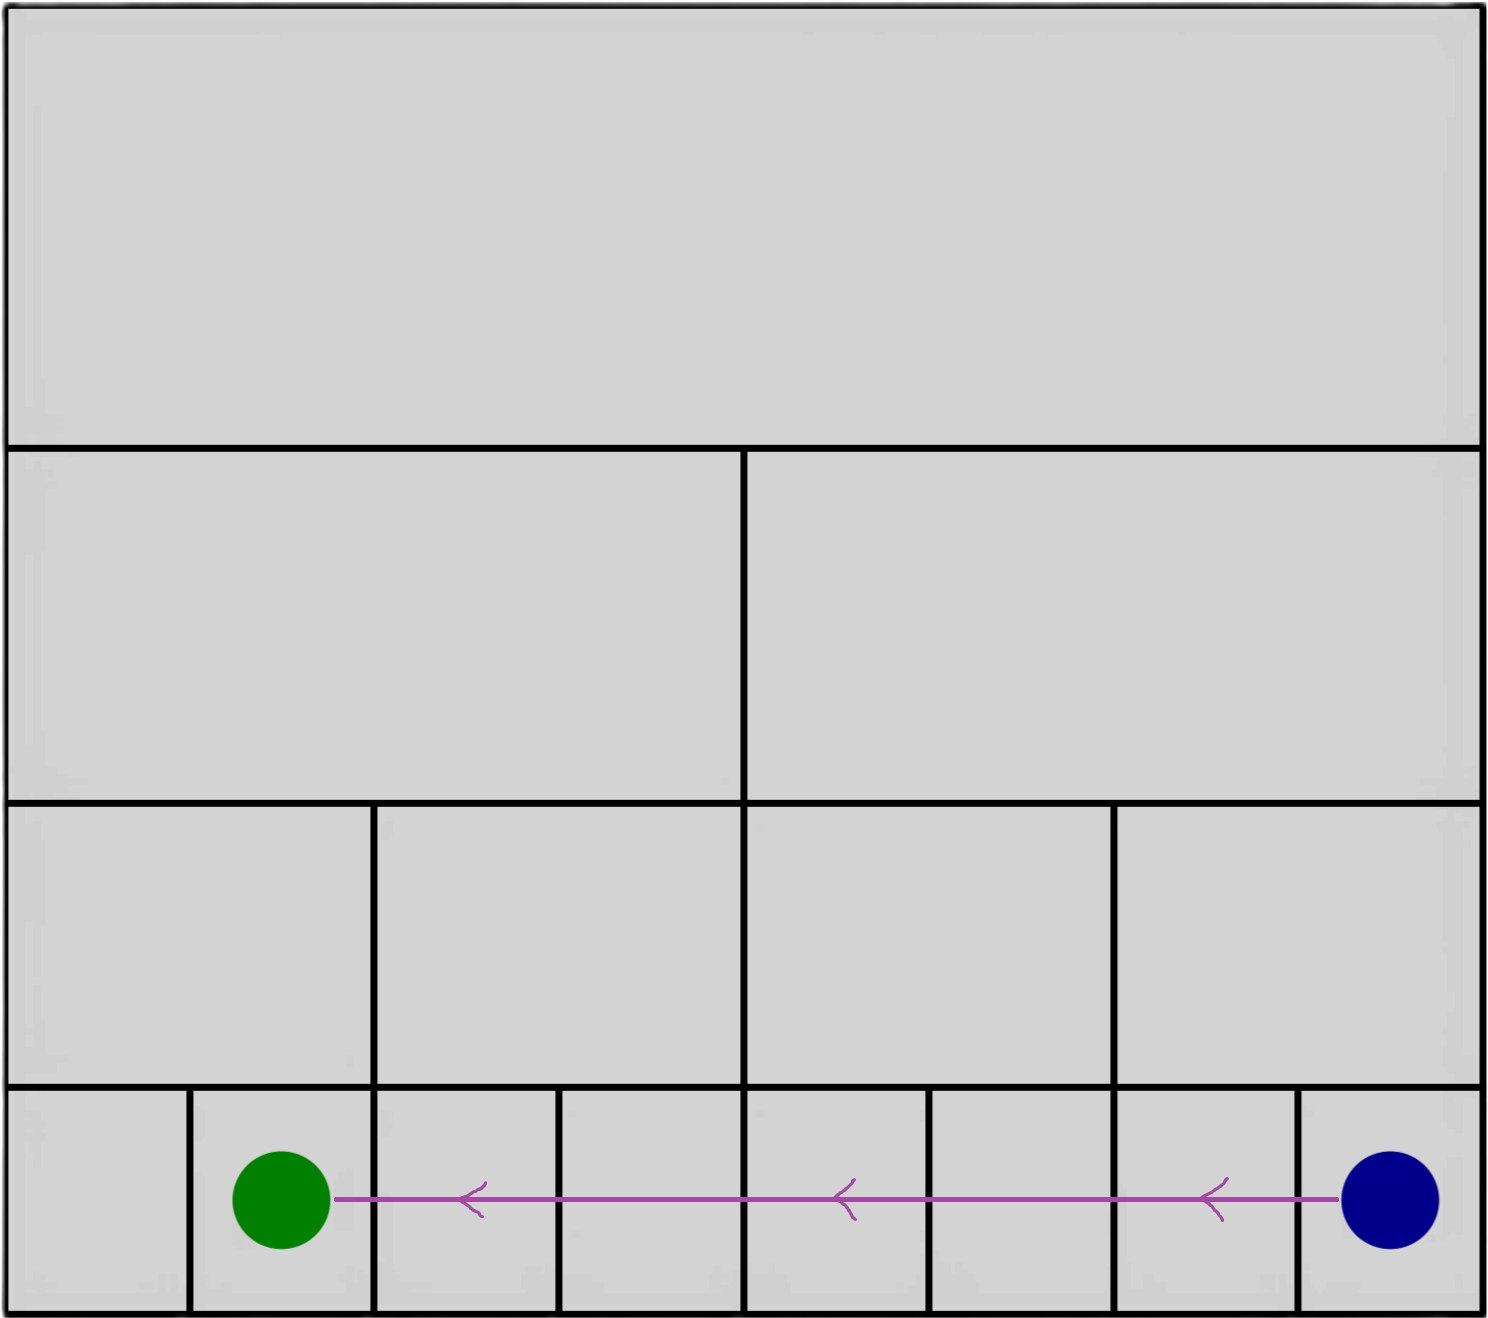
\includegraphics[scale=0.8]{sample2.png}
      \end{subfigure}
      \centering
      \caption{Källarens utseende i exempelfall 1 och exempelfall 2. 
      Den blåa cirkeln markerar var du börjar, och den gröna cirkeln är salen där finalen hålls.
      I båda bilderna är den vägen som Campus Maps hittar markerad lila.
      I exempelfall 1 passerar denna väg tre trappor och en dörr.
      I exempelfall 2 passerar vägen genom noll trappor och sex dörrar.
      }
      \label{fig:samples}
  \end{figure}
\end{centering}

\section*{Interaktion}
Först och främst får du information om rummet du befinner dig i. Detta ges i form av en binär sträng av längd fem,
där varje tecken är ``\texttt{1}'' om du kan gå i en viss riktning och ``\texttt{0}'' annars. I ordning säger strängens tecknen
om du kan gå uppåt, åt höger, nedåt åt höger, nedåt åt vänster, och åt vänster. 
Så strängen \texttt{01001} innebär att det finns ett rum till ditt vänster och ett till ditt höger, 
men inga andra närliggande rum.

Du får sedan välja om du vill gå till ett annat rum, eller använda appen Campus Maps.
För att gå till ett annat rum skriver du någon av strängarna 
``\texttt{up}'', ``\texttt{right}'', ``\texttt{downright}'', ``\texttt{downleft}'' eller ``\texttt{left}''.
Du får då information om det nya rum du befinner dig i, enligt samma format som ovan.

För att använda appen skriver du ``\texttt{app}''. 
Appen beräknar då värdet på $L_v$ enligt beskrivningen ovan.
Eftersom appen är väldigt känslig för Integer Overflows, kommer den krasha om denna längd
överstiger $10^9$. Isåfall skriver appen ut $-1$. Annars skrivs längden på vägen ut. 
När du är framme ska du skriva ut ``\texttt{here}'', och ditt program måste då avslutas.

\textbf{Se till att flusha outputen efter varje query}, annars kan du få \textit{Time Limit Exceeded}.
I C++ kan detta göras med exempelvis \texttt{cout << flush;}
eller \texttt{fflush(stdout);},
i Python med \texttt{stdout.flush()}
och i Java med \texttt{System.out.flush();}.

\section*{Poängsättning}
Din lösning kommer att testas på en mängd testfallsgrupper.
För att få poäng för en grupp så måste du klara alla testfall i gruppen.

\noindent
\begin{tabular}{| l | l | l |}
  \hline
  Grupp & Poängvärde & Gränser \\ \hline \hline
  $1$   & $5$        & $N = 2$ \\ \hline
  $2$   & $10$        & $N \leq 10$ \\ \hline
  $3$   & $10$        & $N \leq 250$ \\ \hline
  $4$   & $16$        & Varje rum som inte ligger längst ner i källaren har två rum under sig. \\ \hline
  $5$   & $13$        & $N \leq 500$ \\ \hline
  $6$   & $21$        & $N \leq 950$ \\ \hline
  $7$   & $25$        & $N \leq 1000$ \\ \hline
\end{tabular}
